\chapter{Integration with Process Simulate}
\label{ch:integration}
\graphicspath{{chapters/Integration/}}

What is process simulate, why we chose it, who uses it and why.

What it allows us to do

Introduce compound operations paths and points

\section{Writing Plug-ins}

how to write a plugin

Tools used and why

\section{Plug-in Architecture}

\section{Plug-in Features}
How to find it in UI

features available

\section{Plug-in Modules}

\section{Optimization Process}

The optimization process consists of the main optimization routine and several modules that provide the required functionality for the algorithm which then glues it together. This chapter will first explain the optimization process and then focus on the supporting modules in the sub-sections. \\

\begin{figure}[ht]
	\caption{Begin Optimization Dialog}
	\centering
	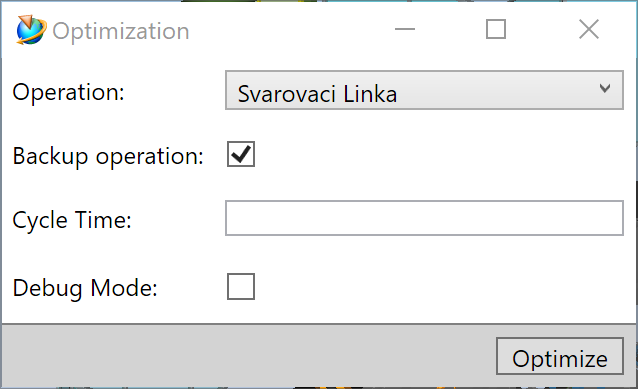
\includegraphics{dialog_beginoptimization}
	\label{fig:DialogBeginOptimization}
\end{figure}

The user first triggers the optimization dialog (see Figure \ref{fig:DialogBeginOptimization}) by clicking on the Optimize button provided by the Plugin. 
The dialog allows the user to adjust parameters of the optimization process. 
First, the system presents him with the operation which should be optimized, which is the operation he had currently set the as the active operation so that he has a chance to adjust this before starting the operation process. In the following text, I will refer to this operation as the root operation.
The user is also presented with the choice to optionally backup the operation which will create a copy of the root operation and then set the duplicate as the new root.
Setting a specific cycle time in seconds will make the MILP model try to match the cycle time instead of minimizing it.
Lastly, the debug option can provide the user with additional information from the MILP solver, explaining the solution, should he have troubles with the proposed schedule. \\

% TODO Class and namespace info

When started, the optimization process will first aim to gather data about the root operation. It will first simulate the behavior of the root operation while the robots are set to maximum and minimum speeds to obtain the minimum and maximum duration of the individual child activities.\\

Then an optimization graph is built by analyzing the operation tree. This graph is also augmented with the information about the simulation and any initial collisions the process might have encountered. After this initial batch of data is gathered the optimization cycle can start. In this loop, the graph is given to a solver which proposes a solution. The process adjusts the root operation to match the proposed solution, and the result is simulated. If there are no collisions, we have the best viable solution, and the cycle ends. Otherwise, we advance to the next round. To prevent an infinite loop, this can only be repeated a limited amount of times. \\

When the process finishes the system will display a helpful report (see Figure \ref{fig:DialogOptimizationResult}) presenting the most important information about the solution to the user. In the header the cycle time can be found and the body is filled with a graphical representation of the schedule.  

\begin{figure}[ht]
	\caption{Optimization Result Dialog}
	\centering
	\includegraphics{}
	\label{fig:DialogOptimizationResult}
\end{figure}

\subsection{Simulation}

The simulation module is a wrapper around the kinematic simulation capability of Process Simulate. It is meant to help with obtaining data about the study which can only be measured. The simulation services are placed in the \emph{Tecnomatix.Optimization.Services.Simulation} and revolve around the \emph{Simulation} class. All new simulations must derive from this class and then can be easily executed. The engine also supports executing multiple simulations simultaneously. \\

To run a simulation, the system needs an operation as an input. Process Simulate will block the UI and compute the movement of the robots in the scope of the given operation, frame by frame. While simulating the player fires events, which the specific simulation can choose to subscribe to if they are relevant for its purpose. Usually, as the playback progresses, the simulation will store some data which when processed will form the output values. Events available range from the simulation being started or ending, operations beginning and ending to the individual time intervals at which the locations of all the objects within the study are computed. \\

A simulation report is a type of simulation, output of which is a data table. This data can be exported into a \emph{csv} file. Reports are useful for debugging or gaining insight into the performance of the activities within the study.

The plugin comes with the following simulations implemented:

\begin{itemize}

\item Collision Simulation. This simulation is checking every frame if there is a collision between the specified collision pairs. The collision pairs can be adjusted in the \emph{Collision Viewer} panel in Process Simulate. The simulation will also track down the responsible operations which controlled the parts that collided.

\item Energy Report. This report captures the simulated energy usage of the robots. Please note that the readings are only as accurate as the robot controller and using a dedicated controller from the manufacturer of the robots is recommended as the readings given by the default robot controller are inaccurate.

\item Joint Speed Report. This report captures the speeds of the joints of the robots while performing the various tasks engulfed in the robotic operation.

\item Duration Simulation. To capture how long it will take for a robot to perform the operation it is first needed for a simulation to run. This information will be captured by Process Simulate afterward, but if any changes happened to the study, it might be inaccurate. For this reason, to obtain accurate readings, this simulation will capture the durations right after the simulation finishes. It is also able to adjust the speed of the robots before running the simulation and restore the original values when done. 

\item Operation Speed Report. This report extracts the speeds the robots are set to run at while executing the particular operations. 

\end{itemize}

\subsection{Graph}

% Class and namespaces
% How it works
% Implemented features

Putting together the optimization graph which serves as the model of the study is one of the most fundamental aspects of the optimization process. It takes a compound operation as an input and traverses all of its descendants transforming it into a flat structure. It also has to analyze the dependencies of the operations and how would it operate in a production cycle. \\

This functionality is being provided by the \emph{GraphVisualizationService} which is located in the \emph{Tecnomatix.Optimization.Services} namespace. It can generate a graph either at bottom-most level of points or one level higher, at the level of paths.

First, the optimization graph is filled with vertexes which are the children of the root operation lying at the desired level, grouped by the robot which is assigned to perform them. In each group, the operations are ordered and a so-called "robot loop" is created, by linking the operations together in pairs, each one with the next. One exception to this rule is the edge between the first and the last operation, which are linked by a "robot loop reset" edge instead.

The hardest part of the graph creation are the "link" edges which can appear at any level in the operation tree. Since we are flattening the tree into a graph, we need to project them into this new structure. 

\subsection{Regulator}

% Class and namespaces
% How it works
% Implemented features

\
